\documentclass[parskip,
							 oneside,
% 							 longdoc,
							 11pt,
							 noheadingspace,
							 accentcolor=tud1d,
							 bigchapter,
							 %draft,
							 colorback]{tudreport}


%% Spracheinstellungen
%\usepackage[ngerman]{babel}
%\usepackage[applemac]{inputenc} % Input-Encodung: applemac fuer Mac
%\IfFileExists{latin1.sty}{\usepackage{latin1}}{\usepackage{isolatin1}}
%\usepackage[latin1]{inputenc}
%\usepackage[T1]{fontenc}
\usepackage[ansinew]{inputenc}  % Input-Encodung: ansinew fuer Windows
\usepackage{microtype} % optischer Randausgleich bei pdflatex mit Zeichendehnung

%% Grafikeinstellungen
\usepackage{float} % u.a. genaue Plazierung von Gleitobjekten mit H
%\usepackage[latin1]{inputenc}


%% Tabelleneinstellungen
\usepackage{booktabs}
\usepackage{multirow}
\usepackage{longtable}
\usepackage{tabularx}

%% State Chart
\usepackage{pgf}
\usepackage{tikz}
\usetikzlibrary{arrows,automata}

%% Mathematik
\usepackage{amsmath}
\usepackage{nicefrac}
\usepackage{icomma}

%% sonstige Einstellungen
\usepackage{paralist}% erweiterte Listenumgebung (z.B. compactitem)
\usepackage{textcomp} % verschiedene Symbole
\usepackage[nottoc, numbib]{tocbibind}
\usepackage{hyperref}
\renewcommand\plparsep{1ex}
\usepackage{enumerate}


\title{\textbf{Computer Systems 2 SoC Lab}}
\subtitle{Report submitted by Julian K\"auser and Fallou Galass Coly}
\subsubtitle{Supervisor: M.Sc. Johanna Rohde\\
			 Begin: Nov. 13th, 2017 \textbar\ Submission: Jan. 15th, 2018\\
			 Institute of Computer Engineering \hfill\textbar\hfill Computer Systems Group \hfill\textbar\hfill Prof.\,Dr.-Ing.\, Christian Hochberger}
\setinstitutionlogo{images/logo.pdf}
% \institution{Institut f\"ur Datentechnik\hfill\textbar\hfill Fachgebiet Rechnersysteme\hfill\textbar\hfill Prof.\,Dr.-Ing.\, Hans Eveking}
%\settitlepicture{images/spartan}
\begin{document}

%% Titel %%%%%%%%%%%%%%%%%%%%%%%%%%%%%%%%%%%%%%%%%%%%%%%%%%%%%%%%%%%%%%%%%%
\maketitle
\cleardoublepage

%% Vorgeplnkel %%%%%%%%%%%%%%%%%%%%%%%%%%%%%%%%%%%%%%%%%%%%%%%%%%%%%%%%%%%%%%
\pagestyle{empty}
%\pagenumbering{roman}
\tableofcontents

%% Hauptteil %%%%%%%%%%%%%%%%%%%%%%%%%%%%%%%%%%%%%%%%%%%%%%%%%%%%%%%%%%%%%%%
\pagestyle{headings}
\pagenumbering{arabic}



\chapter{Introduction}
\label{cha:introduction}

As a part of the \emph{Computer Systems II} lecture, this lab deals with the 
application and driver development for the System-on-Chip (SoC) kit \emph{SpartanMC}, 
which allows the design of an SoC on a FPGA target.
In particular, the task is to generate a system configuration and develop firmware
which allow distance measurements with an ultrasound sensor, a processing of the
measured data, and the view of these results on a connected OLED display. This document
reports about the implementation of the described tasks, and offers insights into the 
development processes. 

The report is structured as following. First, the functions to be implemented are summarized.
Afterwards, the toolchain use is reviewed. Then, 
the generated SoC structure is presented, and the implementations for the utilized 
subsystems are discussed. Before the report is closed with an evaluation of the work, 
a short view on the additional tasks is taken.
\subsubsection{Task Summary}
\label{subsubsec:taskSummary}

As a result of this lab, a SoC system which 
\begin{itemize}
    \item can measure a distance with an ultrasound sensor,
    \item processes the measured data to extinct wrong values and
    \item can display the data on an connected OLED Display.
\end{itemize}

shall be developed. Among the required steps are:
\begin{itemize}
\item Configuring the SoC hardware, including the peripherals for sensor and display 
connections,
\item development of drivers for the SPI and I2C Master,
\item implementation of the protocols of the ultrasound sensor and the OLED display 
driver,
\item design and implementation of a filtering algorithm for  the sensor data and
\item integration of these sub-components into a running system.
\end{itemize}


\section{SpartanMC Toolchain}
\label{sec:spartanMCToolchain}

Developing applications with a SpartanMC system requires the use of the SpartanMC
toolchain. This is a set of applications which must be executed in order to define
the system architecture, develop the firmware and execute it on the hardware. In general,
all tools are triggered by a \emph{make} target in a central makefile; that way, all 
dependency constraints are met. The main tools for the developer are:

\begin{itemize}
\item \textbf{JConfig} \hfill \\
JConfig is a graphical tool to create a new system configuration and add components to
the system. In this task, the used components are a SpartanMC soft core, a clock 
generator, and peripherals conencted to an Advanced Peripheral Bus (APB). More details 
on the system architecture are dscribed in section \ref{sec:systemArchitecture}. 
After the creation of a system configuration, it must be saved. \\
\item \textbf{System Builder} \hfill \\
The SpartanMC System Builder is invoked with the make target \emph{make all program}, 
and reads in the previously designed configuration. It builds the HDL description
of the system, triggers the synthesis of the hardware description, and flashes the 
resulting FPGA configuration onto the target board. As the synthesis and implementation
have to be performed for each system individually, this step requires some time in the
range of seconds to minutes. As long as the hardware is not changed (i.e. no change in 
JConfig), the System Builder does not need to be run again. \\
\item \textbf{Programming the FPGA} \hfill \\
With \emph{make program}, the synthesized hardware design is flashed to the FPGA, as it
is also described in the previous section. Even if the system configuration does not
change, it may be necessary to re-program the FPGA, for example if the FPGA board was 
shut down; the configuration is lost in that case. Although \emph{make program} also writes the
firmware to the memory, this step is further described in the next section.\\
\item \textbf{Programming the Processor} \hfill \\
So far, only hardware is generated. In order to program the processor with the written 
firmware, the code must be compiled, linked and assembled, and be loaded into the memory
of the system. Therefore, the compiler toolchain must be invoked. It compiles the user code
placed in \texttt{firmware/src} and \texttt{firmware/include}, and links it with the 
general libraries wihtin the SpartanMC environment. With \emph{make updateRam program},
the generated executable is transmitted to the memory of the system. The CPU core is 
resetted, and the execution of the user code starts. The target \emph{updateRam} prohibits
the hardware re-configuration and avoids the time-consuming reprogramming process for 
the FPGA target.\\
\item \textbf{Other Tools}\hfill \\
Other than the steps described previously, a serial terminal on the host pc and a logic
analyzer are used. With the serial terminal, status messages and data from the program
can be displayed; additionally, parameters can be sent to the SoC. The logic analyzer 
is helpful to debug electrical problems and can be attached to pins on the target or the 
connected peripherals.
\end{itemize}

As one can see, the central design steps are the configuration of the system architecture
with \emph{JConfig} and writing the user code as \emph{C} code.

\section{System Architecture}
\label{sec:systemArchitecture}
The SoC configuration consists of two major parts: the main system with the cpu core 
and the peripherals. 

For this task, the main system may consist only of one SpartanMC soft core, a memory
block, and a clock generator. This is the minimum configuration, and offers a low complexity.

In order to implement the functions described in the task summary, the SoC requires four 
peripherals: a UART Light Peripheral for serial communication to the host PC, a SPI master 
to send data and commands to the display, an I$^{2}$C master to read out the sensor, 
and a General-Purpose I/O Port, requried to reset the display. These are included in the 
system configuration, as shown in Fig. \ref{fig:SystemArchitecture}.

\begin{figure}
    \centering
    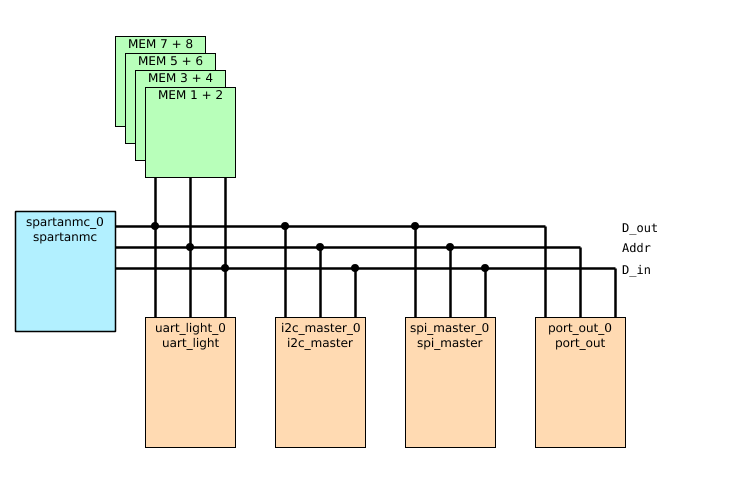
\includegraphics[width=0.9\textwidth]{images/SystemOverview.png}
    \label{fig:SystemArchitecture}
    \caption{System Architecture for the SoC.}
\end{figure}

\section{General Code Structure}
\label{sec:generalCodeStructure}
As a result to this task, several files of C sourcecode have been created. These 
can be split into application code and driver functionality.

The application code consists of the main function (in \texttt{main.c}), which calls
the initializing functions for all modules, and the filter (in \texttt{filter.c/filter.h}).
In the main loop, which is repeated forever, the functions to read the sensor value,
filter it and send it to the display and the host processor are called.

The driver functionality created in this lab is separated into ultrasound sensor reading
procedures (\texttt{ultrasound.c}), SPI sending and init procedures (\texttt{spi.c}), and 
GPIO and I$^{2}$C procedures (\texttt{gpio.c, i2c.c}). The display functions are implemented
in \texttt{oled25664.c}, while a header for this given file had to be added manually.

As presented above, the code structure follows the typical approach for microcontrollers:
first, all peripherals and modules are initialized; in the main loop, abstract driver 
functions are used, so that the concerns for each task are separated.
%\chapter{Toolchain and SoC System}
\label{cha:toolchainAndSystem}

some stuff on the toolchainAndSystem

some stuff on the generated system (block diagram, etc)


\chapter{Inter-Integrated Circuit Bus}
\label{cha:i2c}

some stuff on the i2c interface here
 \chapter{Range Sensor}
 \label{cha:rangeSensor}

The SR02 is a distance sensor based on ultrasound, which 
allows the measurement of distances between 15 centimeters and approximately
six meters. It has an $I^{2}C$ interface, with which it can be started and read 
out. In this chapter, the communication with the sensor via this interface,
as well as the processing of the measured data, is described.

\section{Communication via $I^{2}C$}
\label{sec:sensorI2C}

here some stuff on i2c


\section{Measurement Processing}
\label{sec:filter}

Every measurement performed with sensors is subject to fluctuations, and 
may additionally oly be taken as valid if the values are within the sensors
measuring range. Hence, it is common to apply a processing procedure to 
correct erroneous values. Our filtering procedure is based on two steps, 
as presented in the following.

\subsection{Sensor Range Check}
\label{subsec:sensorRangeCheck}

The SRF02 sensor features a minimum measurable distance of 15 centimeters, 
while the maximum distance is about six meters. Consequently, any value
below the lower threshold or higher than the upper range limit is may not 
be interpreted as valid. Before any further processing, these conditions
are checked; if the currently processed value exceeds the range, it is ignored.
for further processing, the previously stored value from the last measurement 
is used.

\subsection{Median Filter}
\label{subsec:medianFilter}
Before a filter algorithm for measurements can be designed, the unfiltered
data must be examined for errors. Then, an algorithm capable of reducing 
these errors can be developed. 

In our case, we observed two noteable characteristics:

\begin{enumerate}
    \item \textbf{Rogue Results}\hfill \\
    In some cases, especially if the distance is near the lower bound of the 
    sensors range, measured values are wrong because they are much too high.
    For example, when measuring distances between 15 and 20 centimeters, some
    returned values from the sensor are in the range of 200 plus centimeters.
    These have to be filtered out only when the previously measured distances
    clearly indicate that the value around 200 cm cannot be valid.
    \item \textbf{No Distinction at High Error Rate}\hfill \\
    If many measurements are wrong (e.g. below the threshold), it is not possible 
    to determine whether the measured value is right or wrong any more. Hence, the 
    processing can never filter out all errors.
\end{enumerate}

Thus, a filter which stores a number of previous values and determines the 
validity of the current value based on these must be implemented, alothough it can 
never be perfect with this behaviour. A \emph{median filter} is suited well because 
it is capable of sorting out too high or too low, rogue measurements. The filter is 
based on an array, which stores the last $N$ unfiltered values, where $N$ is a 
parameter which must be found fo roptimal filter behaviour. 

For the median filter, three steps are necessary:
\begin{itemize}
    \item First, the oldest value in the array has to be deleted. In our 
    implementation, the oldest value is overwritten by the current measured
    value, and the buffer for the last $N$ values is a ring buffer. Consequently,
    the pointer to the oldest value is incremented, and, if it arrives at the end,
    reset to the initial value.
    \item Second, the buffer with the last $N$ values must be sorted. We chose
    the \emph{Simple Sort} algorithm, which is of $\mathcal{O}(n^{2})$ complexity,
    iterative and works in-place. SpartanMC does not allow too much recursion,
    so an iterative approach is required. The complexity is acceptable for 
    not too large buffers (see section \ref{subsubsec:filterDepth} for 
    details on the choice). As Simple Sort changes the array it is given as 
    input, we decided to copy the buffer array and sort the copy; otherwise,
    the tracking of the order of the last values would be more complex. The 
    complexity of the filter is not changed by the copying process.
    \item At last, the median value must be extracted. If the buffer length is
    odd, the value at \texttt{sorted\_array[length/2 +1]} is used; else, the
    value \texttt{sorted\_array[length/2]} is the median and thus returned.
\end{itemize}

All three steps are performed by separate functions.

\subsubsection{Choice of the Filter Size}
\label{subsubsec:filterDepth}
The number of values taken into account to determine the current filtered 
value is the filter size. Its choice affects the memory demand of the filter,
the computation time per measurement and the quality of the output. 

For our implementation of the median filter, the runtime can be neglected,
 since it will never be longer than the sampling interval of 65 ms. The 
 processor is also not concerned with other demanding tasks.

In our case, two arrays (the one with the measured values and the sorted array)
of the length of the filter have to be allocated. Therefore, the memory demand 
is linear with the filter size.

Finally, the resulting quality of the filter is the key factor for the choice
of its size. With too few previous values, the filter is not able to
neglect many erroneous measurements. A longer filter delays the output of
the corrected value too long, because for every actual larger change of
the distance, more old values have to be replaced. Thus, a larger filter is 
slower; for the median filter, the adaption to a change is even slower than
for e.g. a moving average filter.

after the consideration of these aspects and experiments with the filter size,
we chose a size of 8. In comparison with the unfiltered values, this value
produced acceptably fast changes, while effectively filtering wrong measurements.








\chapter{Serial Peripheral Interface}
\label{cha:spi}

some stuff on spi here
\chapter{OLED Display}
\label{cha:oledDisplay}

some stuff on the display here
\chapter{Additional Tasks}
\label{cha:additionalTasks}

some stuff here why we did not do the extra stuff

\chapter{Evaluation}
\label{cha:evaluation}

some stuff here on perfoirmance, work etc




%% Anhang %%%%%%%%%%%%%%%%%%%%%%%%%%%%%%%%%%%%%%%%%%%%%%%%%%%%%%%%%%%%%%%%
%\appendix
%\bibliographystyle{plain}
%\clearpage
% \nocite{*}
%\bibliography{literaturverzeichnis}


\end{document}
